\subsection{Статистическая модель}

\begin{frame}
\frametitle{Модель цикла}
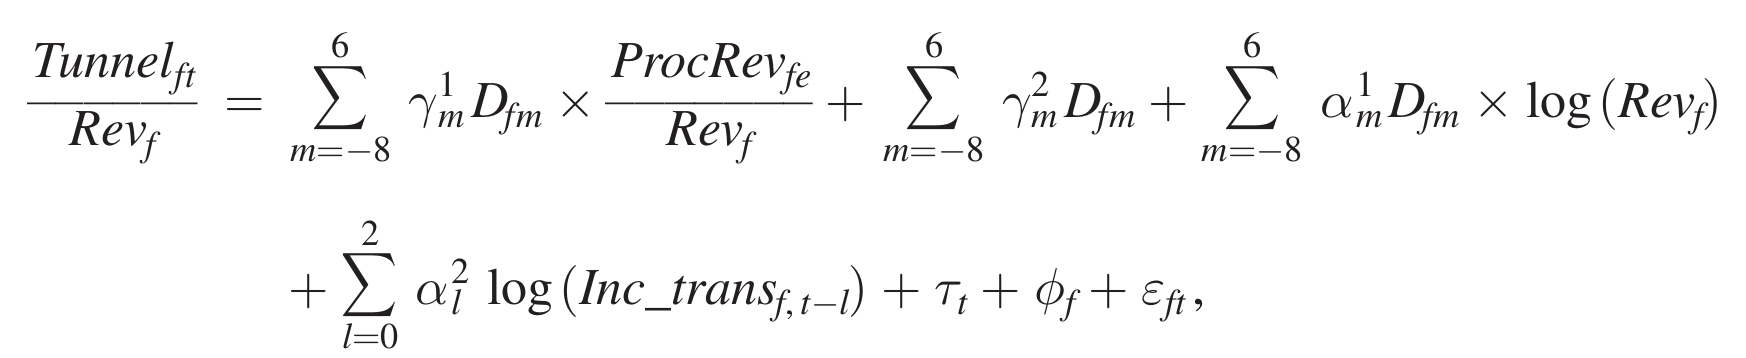
\includegraphics[scale=0.18]{images/cycle2}
\begin{itemize}
	\item $D_{fm}$ - дамми-переменная $m$-го месяца до выборов в регионе фирмы $f$
	\item $ProcRev_{fe}$ - средний годовой доход от гос. заказов для фирмы $f$ в промежутке +-1 года от выборов $e$
	\item $Rev_{f}$ - оборот фирмы $f$ в 2003 году (Росстат)
	\item $Inc\_trans_{f,t}$ - объем входящий трансакций для фирмы $f$ в \\неделю $t$
\end{itemize}
\end{frame}

\begin{frame}
\begin{itemize}
	\item $\gamma^1_m$:\\
		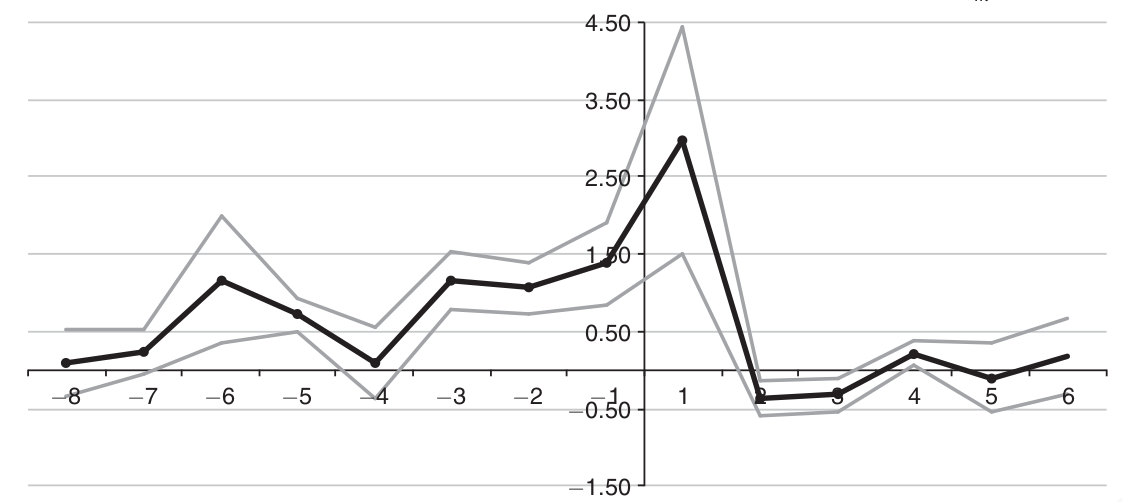
\includegraphics[scale=0.18]{images/el_effect_gamma1}
	
	\item $\gamma^2_m$:\\
		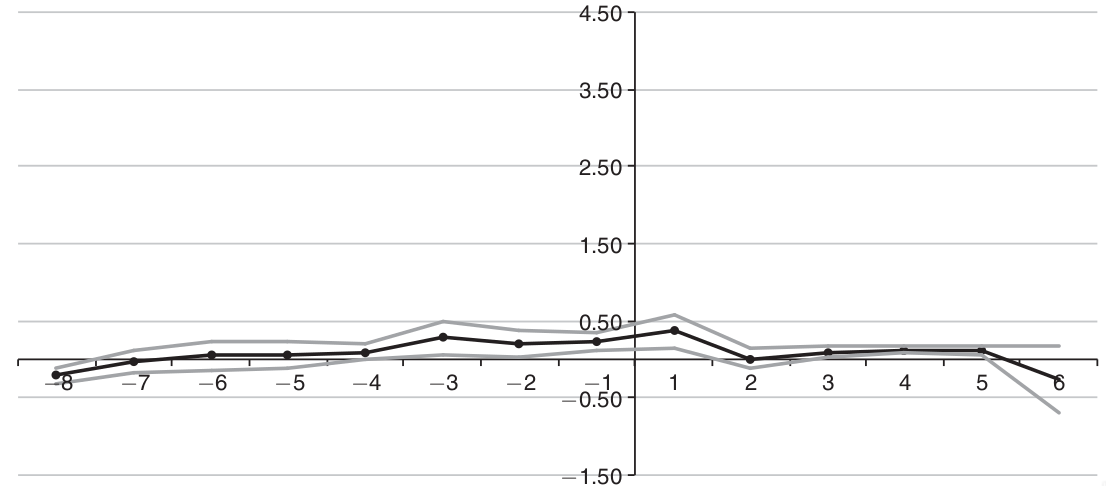
\includegraphics[scale=0.18]{images/el_effect_gamma2}
\end{itemize}
т.е. уеличение доли доходов от гос закупок на 1\% повышает долю выводимых денег на 3\%
\end{frame}


\subsection{Механизм действия}

\begin{frame}
\frametitle{Механизмы влияния выборов на объем выводимых денег}
\begin{itemize}
	
\item Коррупция при розыгрыше тендеров:
	\begin{itemize}
	\item Необходимость подкупить действующее должностное лицо
	\item Необходимость повлиять на выборы в пользу лояльных кандидатов
	\end{itemize}

\item Увеличение экономической активности в целом, которая поднимается, например, вследствие желания текущих должностных лиц быть переизбранными

\item Чувствительность склонности к выводу денег к доходам от гос. заказов

\item Риски, связанные с выборами - изменение политики распределения тендеров
\end{itemize}
\end{frame}
